\chapter{Fourier-Dualität, Impuls und die Bewegung freier Teilchen}

\section{Von den Grundlagen zu Beispielen}

Verschränkung gehört zum Kern der Quantenmechanik. Die Grundlagen sind nun jedoch so weit entwickelt, dass wir sie anwenden können. Bisher stützte sich der Kurs auf bewusst einfache Systeme: einen Spin, einen drehbaren Apparat, eine endliche Liste möglicher Ergebnisse und wiederholte Messungen, aus denen sich Wahrscheinlichkeiten erschließen lassen. Diese Experimente sind logisch einfacher als der historische Weg zur Entdeckung der Quantenmechanik, enthalten aber die nötigen operativen Grundelemente.

\begin{classroomqa}
\audiencequestion{Was entspricht in der Quantenmechanik den wenigen empirischen Ausgangspunkten der Newtonschen Mechanik?}
\lecturerresponse{Ein Minimalmodell ist der drehbare Spinapparat. Man präpariert einen Spin, wählt eine Achse, betätigt die Messvorrichtung, notiert \(+1\) oder \(-1\) und wiederholt das Experiment, bis die Häufigkeiten der Ergebnisse bekannt sind. Der Vektorraum, die Observablen, die Amplituden und die Bornsche Regel ordnen diese Statistik. Historisch entstand die Theorie aus einer viel größeren Vielfalt atomarer Phänomene, doch logisch genügt dieses Experiment mit zwei möglichen Ergebnissen, um ihre Struktur offenzulegen.}
\end{classroomqa}

\begin{classroomqa}
\audiencequestion{Muss dasselbe statistische Verfahren für jede physikalische Größe, etwa Spin oder Impuls, durchgeführt werden?}
\lecturerresponse{Ja. Eine Observable ist an eine Klasse experimenteller Anordnungen und möglicher Ergebnisse gebunden. Der Formalismus sagt die Verteilung voraus, sobald Zustand und Observable festgelegt sind; die physikalische Bedeutung der Observablen ergibt sich jedoch daraus, wie sie gemessen wird.}
\end{classroomqa}

Bevor wir die Verschränkung hinter uns lassen, beantworten wir noch ausführlich eine Frage aus der vorherigen Diskussion. Betrachten wir zwei Elektronen mit Singulett- und Triplettsektoren und beziehen das Strahlungsfeld als weiteres Quantensystem ein. Das Strahlungsfeld hat einen Vakuumzustand \(\ket{0_\gamma}\) und einen Ein-Photon-Zustand \(\ket{1_\gamma}\). Auch die Teilchenzahl kann in einer Überlagerung vorliegen; es gibt keine Regel, die Überlagerungen auf verschiedene Zustände mit fester Teilchenzahl beschränkt.

Für den im Unterricht besprochenen idealisierten Übergang lässt sich ein anfangs unverschränkter Elektronenzustand als Überlagerung von Singulett- und Triplettanteilen schreiben,
\begin{equation}
\ket{\uparrow\downarrow}
=
\frac{1}{\sqrt{2}}
\left(\ket{S}+\ket{T_0}\right).
\end{equation}
Ist anfangs kein Photon vorhanden, lautet der Zustand
\begin{equation}
\ket{\Psi(0)}
=
\frac{1}{\sqrt{2}}
\left(\ket{S}+\ket{T_0}\right)
\otimes\ket{0_\gamma}.
\label{eq:l9-initial-radiative-state}
\end{equation}
Der Singulettanteil bleibt ohne Emission ein Singulett, während der angeregte Triplettanteil in das Singulett relaxieren und ein Photon emittieren kann:
\begin{align}
\ket{S}\ket{0_\gamma}
&\longrightarrow
\ket{S}\ket{0_\gamma}, \\
\ket{T_0}\ket{0_\gamma}
&\longrightarrow
\ket{S}\ket{1_\gamma}.
\end{align}
Aus der Linearität folgt dann
\begin{equation}
\ket{\Psi_{\mathrm{final}}}
=
\ket{S}\otimes
\frac{\ket{0_\gamma}+\ket{1_\gamma}}{\sqrt{2}}.
\label{eq:l9-final-radiative-state}
\end{equation}

\begin{figure}[htbp]
\centering
\includegraphics[width=0.88\textwidth]{lecture_09_figure_01.png}
\caption{Der Elektronenzustand wird in Singulett- und Triplettanteile zerlegt und vor der strahlenden Relaxation mit dem Photonen-Vakuumzustand tensoriert.}
\lectureframe{00:05:10}
\end{figure}

Der Endausdruck ist ein Produktzustand aus dem Elektronenpaar und dem Strahlungsfeld. Die beiden Elektronen sind miteinander verschränkt, denn \(\ket{S}\) ist verschränkt; das Strahlungsfeld befindet sich dagegen in einer Überlagerung aus null und einem Photon. Das Beispiel ist subtil, weil die Wechselwirkung die Verschränkung umverteilt hat: Aus dem anfänglichen Produktzustand der Elektronen entsteht ein verschränktes Elektronenpaar, während der idealisierte Endzustand von Elektronen und Strahlungsfeld ein Produktzustand ist.

\begin{classroomqa}
\audiencequestion{Könnte ein beliebiges einfallendes Photon den Übergang umkehren und die Elektronen entflechten?}
\lecturerresponse{Nein. Der zeitumgekehrte Prozess erfordert den passenden Photonenzustand, Modus, die passende Phase und Energie sowie die entsprechende Wechselwirkungsgeschichte. Das zurückreflektierte emittierte Photon war eine Kurzformulierung dafür, die inverse Entwicklung des gesamten abgeschlossenen Systems herbeizuführen. Es sollte nicht heißen, dass ein beliebiges Photon die Verschränkung aufhebt.}
\end{classroomqa}

\begin{classroomqa}
\audiencequestion{Was veranlasst das Triplett zur Emission, wenn kein äußeres Magnetfeld eingeführt wurde?}
\lecturerresponse{Die Elektronen wechselwirken miteinander und mit dem quantisierten elektromagnetischen Feld. Ihre spinabhängige Wechselwirkung macht eine der Spin-Konfigurationen energetisch günstiger; die überschüssige Energie kann als Strahlung abgegeben werden. Dazu ist kein äußeres Messgerät nötig: Es handelt sich um die gewöhnliche unitäre Dynamik des Gesamtsystems aus Elektronen und Feld.}
\end{classroomqa}

Nachdem wir diesen letzten Punkt geklärt haben, lassen wir den Spin nun außer Betracht und untersuchen das einfachste Bewegungsproblem: ein Teilchen auf einer eindimensionalen Geraden.

\section{Ebenen Wellen und das Fourier-Paar}

Bevor wir zur Physik zurückkehren, schieben wir einen mathematischen Exkurs ein. Wir beginnen mit
\begin{equation}
e^{ipx}=\cos(px)+i\sin(px).
\end{equation}
In diesem Stadium ist \(p\) einfach eine reelle Zahl, die die Oszillationsrate bestimmt. Der Ausdruck hängt nicht von der Zeit ab und beschreibt daher noch keine laufende Welle. Man nennt ihn ebene Welle, weil er als Funktion von \(x\) die vertraute Sinusform hat.

Eine große Klasse hinreichend regulärer Funktionen lässt sich in solche Moden zerlegen. Wir betrachten Funktionen, die sich für die folgenden Integrale ausreichend gut verhalten: Sie dürfen im räumlichen Unendlichen nicht divergieren, und die späteren physikalischen Wellenfunktionen müssen quadratintegrabel sein. Bei symmetrischer Normierung lautet das Fourier-Paar
\begin{align}
\psi(x)
&=
\int_{-\infty}^{\infty}
\frac{dp}{\sqrt{2\pi}}\,
\widetilde{\psi}(p)e^{ipx},
\label{eq:l9-fourier-forward}\\
\widetilde{\psi}(p)
&=
\int_{-\infty}^{\infty}
\frac{dx}{\sqrt{2\pi}}\,
\psi(x)e^{-ipx}.
\label{eq:l9-fourier-inverse}
\end{align}
Der Koeffizient \(\widetilde{\psi}(p)\) ist die komplexe Amplitude der Mode mit dem Fourier-Parameter \(p\). Die Faktoren \(1/\sqrt{2\pi}\) sind Konvention; steht in jeder Richtung einer, sehen die beiden Formeln zueinander reziprok aus. Das relative Minuszeichen im Exponenten ist wesentlich.

\begin{figure}[htbp]
\centering
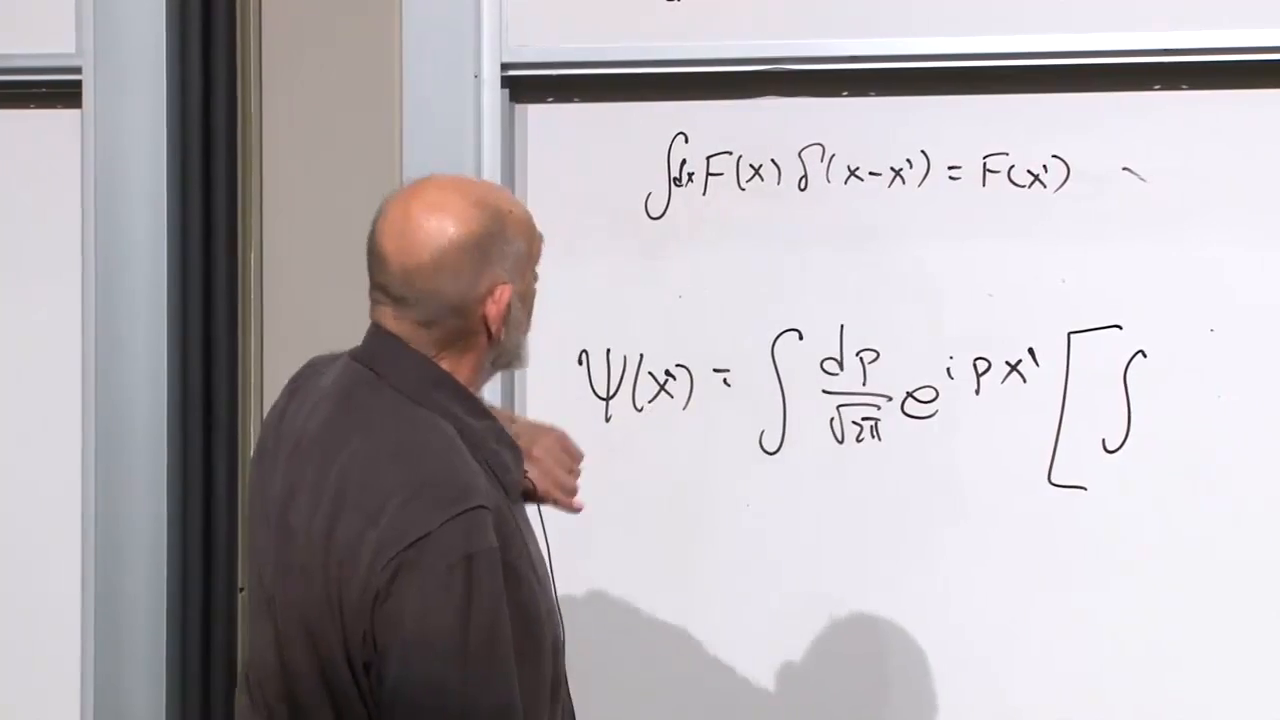
\includegraphics[width=0.88\textwidth]{lecture_09_figure_02.png}
\caption{Das symmetrische Fourier-Paar: Eine Funktion wird in ebene Wellen zerlegt, und die Modenamplituden erhält man durch die inverse Transformation.}
\lectureframe{00:14:35}
\end{figure}

\begin{classroomqa}
\audiencequestion{Sind \(\psi(x)\) und \(\widetilde{\psi}(p)\) als komplexe Größen gemeint?}
\lecturerresponse{Im Allgemeinen ja. Eine spezielle Funktion kann zufällig reell sein; dann erfüllen ihre Fourier-Koeffizienten eine zusätzliche Konjugationsrelation. Quantenamplituden sind jedoch von Natur aus komplex, und hier wird keine Einschränkung auf reelle Funktionen gemacht.}
\end{classroomqa}

\begin{classroomqa}
\audiencequestion{Warum verwendet man die symmetrischen Faktoren \(1/\sqrt{2\pi}\), statt den gesamten Faktor \(2\pi\) in eine der beiden Transformationen zu legen?}
\lecturerresponse{Beide Konventionen sind konsistent. Bei der symmetrischen Wahl unterscheiden sich Vorwärts- und Rücktransformation nur durch das Vorzeichen im Exponenten. Physikalische Vorhersagen hängen nicht von der Konvention ab, sofern alle damit verbundenen Normierungen konsistent angepasst werden.}
\end{classroomqa}

Die reziproke Beziehung zwischen \(x\) und \(p\) ist bereits erkennbar. Eine Funktion lässt sich durch Integration über die jeweils andere Variable darstellen. Im Moment ist das Fourier-Analysis. Bald wird dasselbe Paar für Ort und Impuls stehen.

\section{Die Dirac-Deltafunktion als Operation}

Anschaulich ist die Deltafunktion ein Spike mit verschwindender Breite, unbeschränkter Höhe und Flächeninhalt eins. Dieses Bild ist nützlich, doch die operationale Definition ist verlässlicher. Für jede geeignete Testfunktion \(f\) gilt
\begin{equation}
\int_{-\infty}^{\infty}
dx\,\delta(x-x')f(x)
=f(x').
\label{eq:l9-delta-sampling}
\end{equation}
Drei bekannte Regeln bringen dieselbe Idee zum Ausdruck:
\begin{align}
f(x)\delta(x-x')
&=
f(x')\delta(x-x'),
\label{eq:l9-delta-multiplication}\\
\int_{-\infty}^{\infty}dx\,\delta(x-x')
&=1,
\label{eq:l9-delta-area}\\
\int_{-\infty}^{\infty}dx\,\delta(x-x')f(x)
&=f(x').
\end{align}
Die erste Regel gilt, weil die Deltafunktion nur bei \(x=x'\) Träger hat. In der zweiten Regel verschiebt sich der Spike, doch sein Flächeninhalt bleibt gleich. Aus diesen beiden Regeln folgt die dritte.

\begin{figure}[htbp]
\centering
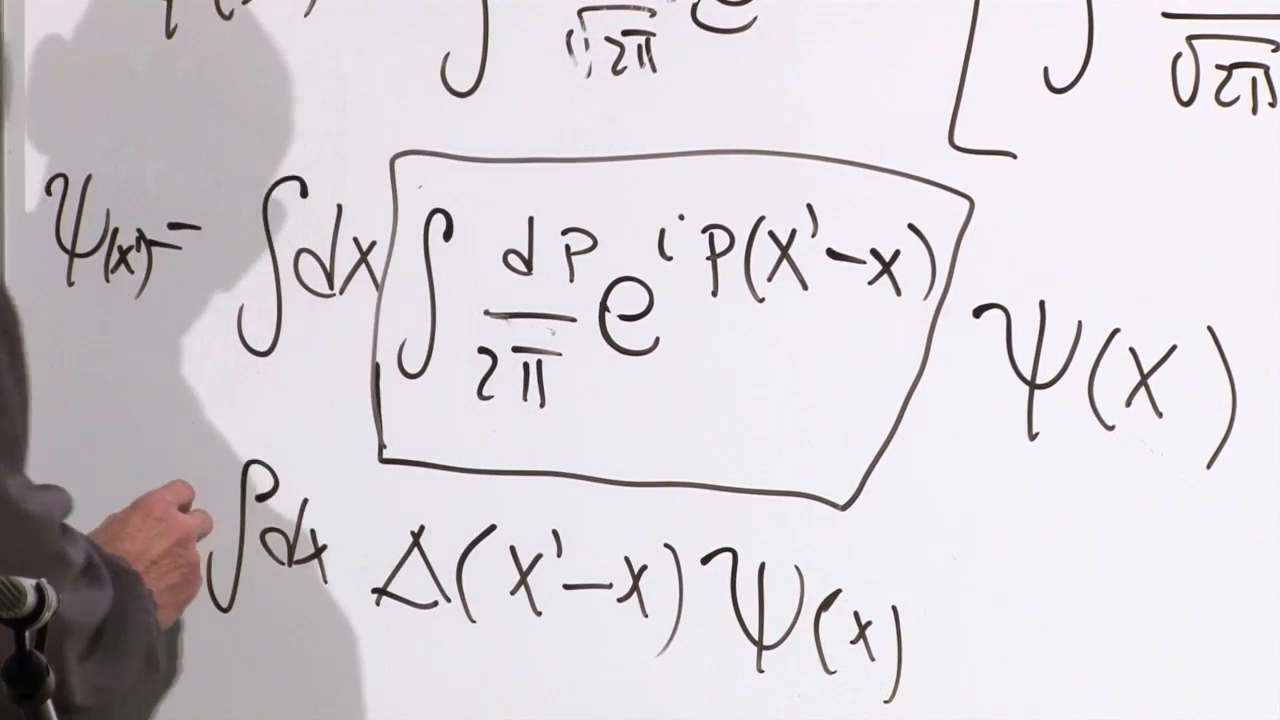
\includegraphics[width=0.88\textwidth]{lecture_09_figure_03.png}
\caption{Die Abtasteigenschaft charakterisiert die Dirac-Deltafunktion durch ihre Wirkung auf jede geeignete Funktion.}
\lectureframe{00:19:45}
\end{figure}

\begin{classroomqa}
\audiencequestion{Warum kann \(f(x')\) aus dem \(x\)-Integral herausgezogen werden?}
\lecturerresponse{Die Integrationsvariable ist \(x\). Der Parameter \(x'\) bleibt während dieser Integration fest, daher ist \(f(x')\) bezüglich \(x\) konstant. Das verbleibende Delta-Integral hat den Flächeninhalt eins.}
\end{classroomqa}

Die Deltafunktion ist keine gewöhnliche punktweise Funktion. Insbesondere führt ihr Quadrieren auf ein Objekt, das noch singulärer ist als die Deltafunktion selbst. Ihre wohldefinierte Bedeutung ist distributionell: Gleichung~\eqref{eq:l9-delta-sampling} legt fest, wie sie unter einem Integral wirkt.

\subsection{Die Fourier-Darstellung der Deltafunktion}

Setzen wir Gleichung~\eqref{eq:l9-fourier-inverse} in Gleichung~\eqref{eq:l9-fourier-forward} ein und benennen das Argument auf der linken Seite in \(x'\) um:
\begin{align}
\psi(x')
&=
\int\frac{dp}{\sqrt{2\pi}}\,
e^{ipx'}
\left[
\int\frac{dx}{\sqrt{2\pi}}\,
\psi(x)e^{-ipx}
\right] \notag\\
&=
\int dx
\left[
\int\frac{dp}{2\pi}
e^{ip(x'-x)}
\right]\psi(x).
\label{eq:l9-fourier-composition}
\end{align}
Der Ausdruck in eckigen Klammern muss für jede geeignete Funktion \(\psi\) den Wert \(\psi(x')\) ergeben. Vergleichen wir dies mit der definierenden Wirkung der Deltafunktion, erhalten wir
\begin{equation}
\boxed{
\int_{-\infty}^{\infty}
\frac{dp}{2\pi}\,
e^{ip(x'-x)}
=\delta(x'-x)
}.
\label{eq:l9-delta-fourier-x}
\end{equation}

\begin{figure}[htbp]
\centering
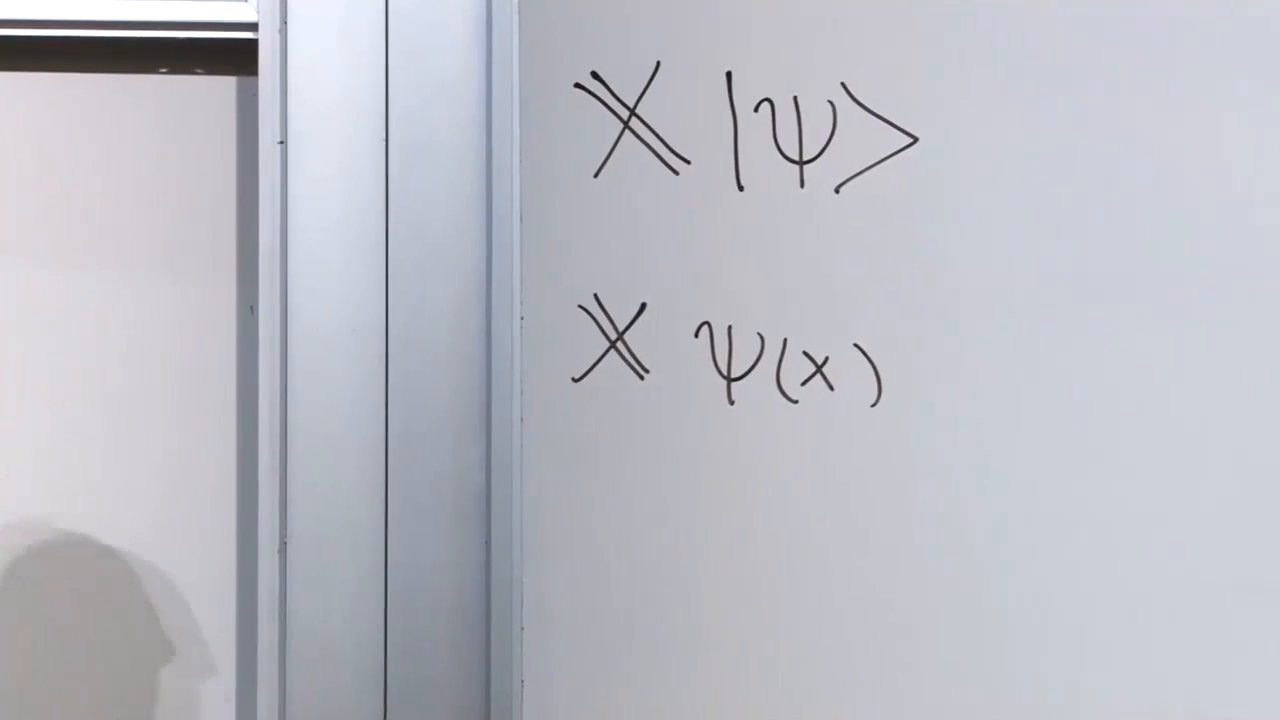
\includegraphics[width=0.88\textwidth]{lecture_09_figure_04.png}
\caption{Der Fourier-Kern wird in der Verkettung der beiden Transformationen isoliert und anhand seiner Abtasteigenschaft als Dirac-Deltafunktion identifiziert.}
\lectureframe{00:26:23}
\end{figure}

Vertauscht man die Bezeichnungen der reziproken Variablen, erhält man die entsprechende Identität
\begin{equation}
\boxed{
\int_{-\infty}^{\infty}
\frac{dx}{2\pi}\,
e^{ix(p-p')}
=\delta(p-p')
}.
\label{eq:l9-delta-fourier-p}
\end{equation}
Die Deltafunktion ist somit eine kontinuierliche Überlagerung ebener Wellen.

\begin{classroomqa}
\audiencequestion{Der Exponent wurde einmal als \(x'-x\) und an anderer Stelle als \(x-x'\) geschrieben. Ändert das Vorzeichen das Ergebnis?}
\lecturerresponse{Nein. Die Deltafunktion ist gerade: \(\delta(u)=\delta(-u)\). Daher ändert eine Umkehrung des Vorzeichens der Differenz die resultierende Distribution nicht. Der Exponentialterm dazwischen wird zwar komplex konjugiert, aber der integrierte Kern ergibt dieselbe Deltafunktion.}
\end{classroomqa}

Bei diesen Umformungen wird eine Konvergenzeinschränkung übergangen. Die oszillierenden Integrale sind Distributionen und keine gewöhnlichen, absolut konvergenten Integrale; auch das Vertauschen der Integrationsreihenfolge erfordert Sorgfalt. Ein endliches periodisches Intervall liefert einen sauberen Regulator: Zunächst verwendet man diskrete Fourier-Moden und die Orthogonalität des Kronecker-Deltas, dann lässt man das Intervall unbegrenzt anwachsen. Die obigen Kontinuumsidentitäten ergeben sich als Grenzfall.

\section{Ein Teilchen auf einer Geraden}

Klassisch legt ein einzelner Punkt im Phasenraum den Zustand fest:
\begin{equation}
(x,p).
\end{equation}
Die Quantenmechanik stellt zunächst eine andere Frage: Welche Orthonormalbasis definiert den Zustandsraum? Zu jedem reellen Ort \(x\) führen wir einen verallgemeinerten Eigenket \(\ket{x}\) ein. Ein allgemeiner Zustand lässt sich entwickeln als
\begin{equation}
\ket{\Psi}
=
\int_{-\infty}^{\infty}
dx\,\psi(x)\ket{x},
\qquad
\psi(x)=\braket{x}{\Psi}.
\label{eq:l9-position-expansion}
\end{equation}

\begin{figure}[htbp]
\centering
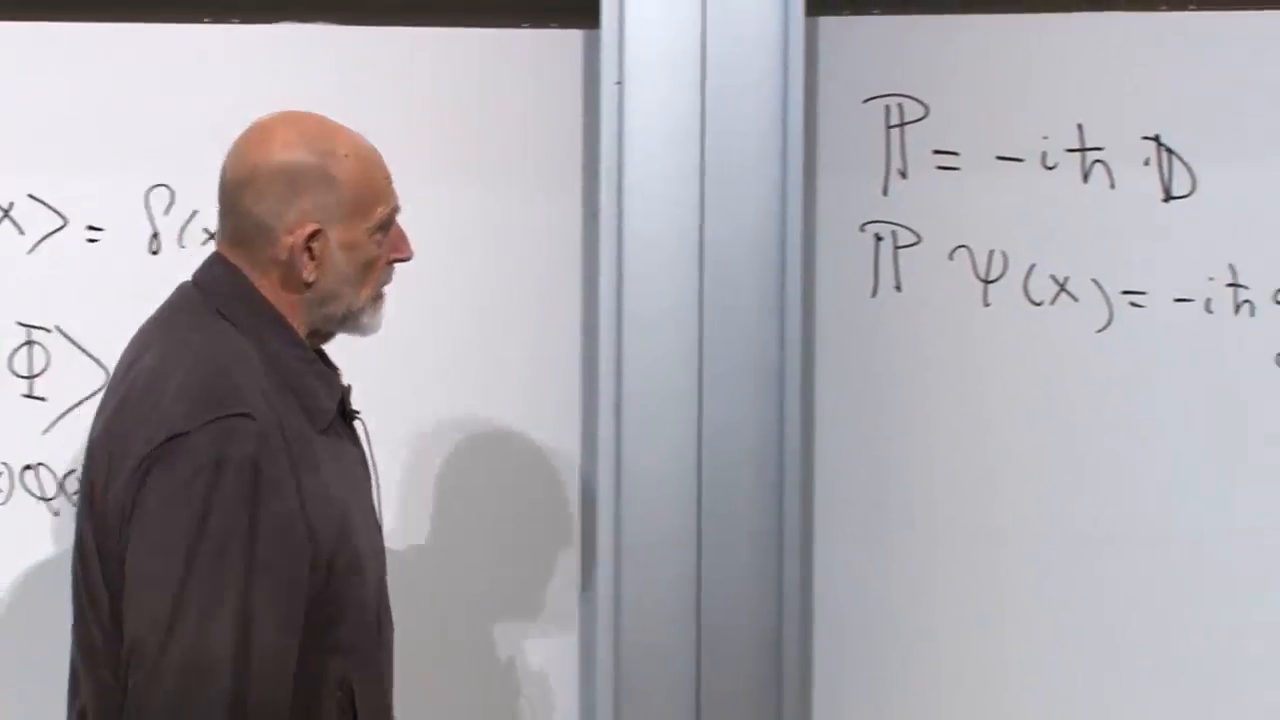
\includegraphics[width=0.88\textwidth]{lecture_09_figure_05.png}
\caption{Ein allgemeiner Zustand in der kontinuierlichen Ortsbasis entwickelt; der Koeffizient ergibt sich durch Projektion auf \(\ket{x}\).}
\lectureframe{00:35:30}
\end{figure}

Die Bornsche Regel ordnet die Wahrscheinlichkeitsdichte zu:
\begin{equation}
\rho(x)=|\psi(x)|^2.
\end{equation}
Die Wahrscheinlichkeit in einem endlichen Intervall ist
\begin{equation}
P(a<x<b)=\int_a^b|\psi(x)|^2\,dx,
\end{equation}
und ein normierter physikalischer Zustand erfüllt
\begin{equation}
\int_{-\infty}^{\infty}|\psi(x)|^2\,dx=1.
\label{eq:l9-position-normalization}
\end{equation}
Die kontinuierliche Orthogonalität wird ausgedrückt durch
\begin{equation}
\braket{x'}{x}=\delta(x-x').
\label{eq:l9-position-delta}
\end{equation}
Für zwei beliebige Zustände lautet das Skalarprodukt
\begin{equation}
\braket{\Psi}{\Phi}
=
\int_{-\infty}^{\infty}
dx\,\psi^*(x)\phi(x).
\label{eq:l9-position-inner-product}
\end{equation}

\begin{figure}[htbp]
\centering
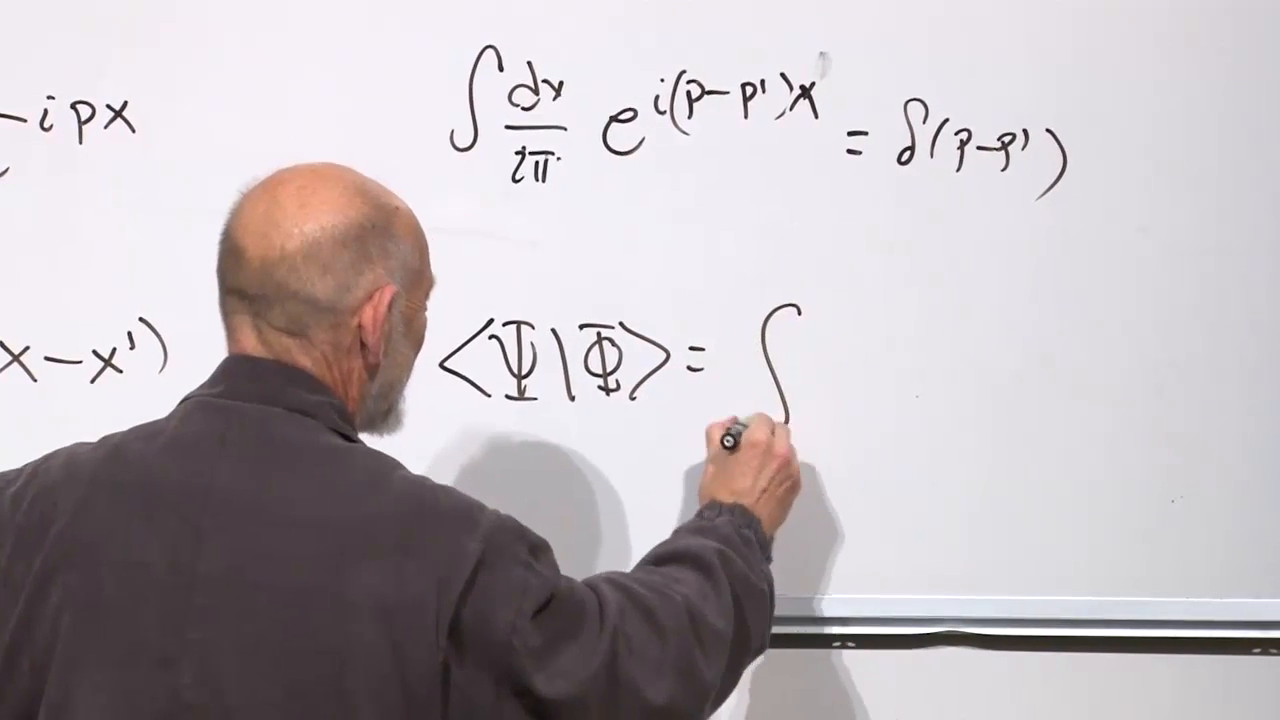
\includegraphics[width=0.88\textwidth]{lecture_09_figure_06.png}
\caption{Die Normierung der kontinuierlichen Basis und das Wellenfunktions-Skalarprodukt in der Ortsdarstellung.}
\lectureframe{00:41:20}
\end{figure}

\begin{classroomqa}
\audiencequestion{Warum genügt der Ort allein? Wäre es überflüssig, den Impuls oder fast jede andere Variable hinzuzufügen?}
\lecturerresponse{Für ein Teilchen in einer Dimension legt die vollständige Funktion \(\psi(x)\) den Zustand fest; ein zugleich scharfer Wert von \(p\) wäre also eine übermäßige Festlegung. Der Impuls liefert eine weitere vollständige Basis, statt ein zusätzliches Etikett für jedes \(\ket{x}\) zu sein. In mehreren Dimensionen lassen sich kompatible Größen kombinieren: Zum Beispiel kommutieren \(X\) und \(P_y\) und können eine gemeinsame Basis kennzeichnen. Die Einschränkung betrifft nichtkommutierende Paare, sondern nicht einfach die Anzahl der Symbole.}
\end{classroomqa}

\begin{classroomqa}
\audiencequestion{Kann auch der Impuls eine vollständige Basis liefern, und lässt sich der Zustand über den Ort entwickeln?}
\lecturerresponse{Ja. Die Impulsbasis ist vollständig, und ihre Koeffizienten sind durch Fourier-Transformation mit den Ortskoeffizienten verknüpft. Diese Beziehung ist die zentrale Konstruktion dieser Vorlesung.}
\end{classroomqa}

\section{Der Ort in der Ortsdarstellung}

Ein abstrakter Operator wirkt auf Zustandsvektoren. Sobald eine Basis gewählt ist, wird dieselbe Wirkung zu einer konkreten Operation auf Wellenfunktionen. In der Ortsdarstellung wirkt der Ortsoperator \(X\) durch Multiplikation:
\begin{equation}
(X\psi)(x)=x\psi(x).
\label{eq:l9-position-operator}
\end{equation}

Der bei \(x_0\) lokalisierte Zustand wird durch die verallgemeinerte Wellenfunktion \(\delta(x-x_0)\) dargestellt. Wenden wir \(X\) an, so erhalten wir
\begin{align}
X\delta(x-x_0)
&=
x\delta(x-x_0) \notag\\
&=
x_0\delta(x-x_0),
\label{eq:l9-position-eigenfunction}
\end{align}
wobei Gleichung~\eqref{eq:l9-delta-multiplication} verwendet wurde. Damit ist \(\delta(x-x_0)\) eine Eigenfunktion von \(X\) zum Eigenwert \(x_0\).

\begin{figure}[htbp]
\centering
\includegraphics[width=0.88\textwidth]{lecture_09_figure_07.png}
\caption{Die Multiplikation mit \(x\) macht aus dem delta-lokalisierten Zustand \(x_0\) mal sich selbst und zeigt damit, dass er eine Orts-Eigenfunktion ist.}
\lectureframe{00:45:50}
\end{figure}

Weder \(\ket{x_0}\) noch seine Darstellung durch eine Deltafunktion ist im gewöhnlichen quadratintegrablen Sinn auf eins normiert. Er ist delta-normalisiert. Physikalische lokalisierte Zustände sind endliche Wellenpakete, während exakte Eigenzustände als verallgemeinerte Basisvektoren dienen.

\section{Impuls-Eigenfunktionen}

In der vorherigen Vorlesung wurde gezeigt, dass Differentiation antihermitesch ist und Multiplikation mit \(-i\) sie hermitesch macht. Unter Berücksichtigung der Einheiten definieren wir
\begin{equation}
P=-i\hbar\frac{d}{dx},
\qquad
(P\psi)(x)
=
-i\hbar\frac{d\psi}{dx}.
\label{eq:l9-momentum-operator}
\end{equation}
Dies ist eine zulässige Observable auf einem geeigneten Definitionsbereich. Ob sie mit dem physikalischen Impuls identifiziert werden kann, prüfen wir anhand ihres Spektrums, ihrer Wellenlänge und ihrer Rolle in der Dynamik.

Für einen Impuls-Eigenwert \(p\) lösen wir
\begin{equation}
P\psi_p=p\psi_p,
\end{equation}
oder
\begin{equation}
-i\hbar\frac{d\psi_p}{dx}=p\psi_p.
\end{equation}
Die Lösung lautet
\begin{equation}
\psi_p(x)=A e^{ipx/\hbar}.
\label{eq:l9-momentum-eigenfunction}
\end{equation}

\begin{figure}[htbp]
\centering
\includegraphics[width=0.88\textwidth]{lecture_09_figure_08.png}
\caption{Die Ortsraumdarstellung eines Zustands mit bestimmtem Impuls ist eine ebene Welle \(e^{ipx/\hbar}\).}
\lectureframe{00:51:45}
\end{figure}

Die Wellenlänge \(\lambda\) ist die Verschiebung, die die Phase um \(2\pi\) anwachsen lässt:
\begin{equation}
\frac{p\lambda}{\hbar}=2\pi,
\qquad
\lambda=\frac{2\pi\hbar}{p}.
\label{eq:l9-de-broglie}
\end{equation}
Ein größerer Impuls entspricht daher einer kürzeren Wellenlänge.

Die Delta-Normierung legt die Konstante fest:
\begin{equation}
\psi_p(x)
=
\frac{1}{\sqrt{2\pi\hbar}}e^{ipx/\hbar}.
\label{eq:l9-normalized-momentum-eigenfunction}
\end{equation}
Tatsächlich gilt
\begin{align}
\braket{p'}{p}
&=
\int_{-\infty}^{\infty}
dx\,
\psi_{p'}^*(x)\psi_p(x) \notag\\
&=
\int_{-\infty}^{\infty}
\frac{dx}{2\pi\hbar}
e^{i(p-p')x/\hbar} \notag\\
&=
\delta(p-p').
\label{eq:l9-momentum-normalization}
\end{align}
Wählt man Einheiten mit \(\hbar=1\), so werden diese Formeln zu
\begin{equation}
\psi_p(x)=\frac{1}{\sqrt{2\pi}}e^{ipx},
\qquad
\int\frac{dx}{2\pi}e^{i(p-p')x}
=\delta(p-p').
\end{equation}

\begin{classroomqa}
\audiencequestion{Wie kann man das oszillierende Integral für \(p\neq p'\) gleich null setzen, obwohl es im gewöhnlichen Sinn nicht konvergiert?}
\lecturerresponse{Die Vorlesung verwendet hier eine kontrollierte Abkürzung. Man legt das System auf ein endliches periodisches Intervall. Die zulässigen Impulse bilden dann eine diskrete Menge, die Exponentialfunktionen sind im gewöhnlichen Sinn orthogonal und alle Normierungen endlich. Erst nach dieser Rechnung lässt man das Intervall gegen unendlich gehen; dabei wird aus dem Kronecker-Delta eine Dirac-Deltafunktion.}
\end{classroomqa}

\begin{classroomqa}
\audiencequestion{Betrifft dasselbe Konvergenzproblem auch die Herleitung der Deltafunktion mithilfe der Fourier-Transformation?}
\lecturerresponse{Ja. Auch dort war das Vertauschen der Integrationen aus demselben Grund formal. Die Herleitung in einem endlichen Kasten oder die Sprache der Distributionen liefert die ausgelassene Begründung. Diese Abkürzung ist vertretbar, weil die regulierte Rechnung den angegebenen Kontinuumsgrenzwert hat.}
\end{classroomqa}

\section{Die Impulsdarstellung}

Zwei Dinge dürfen nicht verwechselt werden. Die Funktion \(\psi_p(x)\) in Gleichung~\eqref{eq:l9-normalized-momentum-eigenfunction} ist die Ortsraumdarstellung des speziellen Eigenzustands \(\ket{p}\). Die Impulsraum-Wellenfunktion eines beliebigen Zustands \(\ket{\Psi}\) ist dagegen
\begin{equation}
\widetilde{\psi}(p)=\braket{p}{\Psi}.
\label{eq:l9-momentum-wavefunction}
\end{equation}
Setzen wir die Ortsraum-Wellenfunktionen von \(\bra{p}\) und \(\ket{\Psi}\) ein:
\begin{align}
\widetilde{\psi}(p)
&=
\int_{-\infty}^{\infty}
dx\,
\braket{p}{x}\braket{x}{\Psi} \notag\\
&=
\int_{-\infty}^{\infty}
\frac{dx}{\sqrt{2\pi\hbar}}\,
e^{-ipx/\hbar}\psi(x).
\label{eq:l9-position-to-momentum}
\end{align}
Das ist genau die Fourier-Transformation. Umgekehrt gilt
\begin{equation}
\psi(x)
=
\int_{-\infty}^{\infty}
\frac{dp}{\sqrt{2\pi\hbar}}\,
\widetilde{\psi}(p)e^{ipx/\hbar}.
\label{eq:l9-momentum-to-position}
\end{equation}

\begin{figure}[htbp]
\centering
\includegraphics[width=0.88\textwidth]{lecture_09_figure_09.png}
\caption{Die Projektion auf \(\ket{p}\) macht aus der Ortsraum-Wellenfunktion ihre Fourier-Transformierte \(\widetilde{\psi}(p)\).}
\lectureframe{01:05:50}
\end{figure}

Die Wahrscheinlichkeitsdichte für eine Impulsmessung mit Ergebnis \(p\) ist
\begin{equation}
\widetilde{\rho}(p)
=
|\widetilde{\psi}(p)|^2,
\qquad
\int_{-\infty}^{\infty}
|\widetilde{\psi}(p)|^2\,dp=1.
\end{equation}
Eine einzige Ortsraum-Wellenfunktion enthält somit genügend Information, um sowohl Orts- als auch Impulsmessungen vorherzusagen. Um die Impulswahrscheinlichkeiten zu bestimmen, transformiert man \(\psi(x)\) fourier und bildet den Betrag des Ergebnisses zum Quadrat.

In der Impulsdarstellung kehren sich die Rollen um:
\begin{equation}
(P\widetilde{\psi})(p)
=
p\widetilde{\psi}(p),
\qquad
(X\widetilde{\psi})(p)
=
i\hbar\frac{d\widetilde{\psi}}{dp}.
\label{eq:l9-operators-in-p}
\end{equation}
Das Vorzeichen unterscheidet sich von \(P=-i\hbar\,d/dx\) wegen der entgegengesetzten Vorzeichen im Fourier-Paar.

\begin{classroomqa}
\audiencequestion{Ist die Zeit wie der Ort zum Impuls der Energie konjugiert?}
\lecturerresponse{Die Zeit wird gewöhnlich als äußerer Parameter behandelt, der die Zustandsentwicklung beschreibt, nicht als universeller selbstadjungierter Operator auf dem Hilbertraum des Systems. Eine physikalische Uhr hat durchaus beobachtbare Anzeigen, und eine höhere Zeitauflösung der Uhr hat Folgen für die Energie. Die Zeit-Energie-Beziehung erfordert jedoch mehr Sorgfalt als das Ort-Impuls-Paar und wird hier nicht behandelt.}
\end{classroomqa}

\begin{classroomqa}
\audiencequestion{Welche anderen konjugierten Paare gibt es?}
\lecturerresponse{Winkel und der zugehörige Drehimpuls sind ein wichtiges Beispiel, wobei sich aus der Periodizität des Winkels globale Einschränkungen ergeben. In der Feldtheorie sind ein Feld und sein kanonischer Impuls konjugiert. Temperatur und Druck sind thermodynamische Variablen, kein kanonisches quantenmechanisches Paar. Das allgemeine Prinzip folgt aus kanonischen Variablen und ihren Kommutatoren, nicht aus beliebigen Paaren messbarer Größen.}
\end{classroomqa}

\begin{classroomqa}
\audiencequestion{Wirken Operatoren in der diskreten Theorie auf Kets, während Wellenfunktionen nur Koeffizienten auflisten. Ist das in der kontinuierlichen Theorie anders?}
\lecturerresponse{Nein. Eine Wellenfunktion ist die Koordinatenspalte eines abstrakten Kets in einer gewählten Basis. Eine Matrix, die auf eine endliche Spalte wirkt, und ein Differential- oder Integraloperator, der auf eine Funktion wirkt, sind zwei konkrete Darstellungen derselben abstrakten Operation. Das kontinuierliche Etikett ändert die Notation, nicht die Logik.}
\end{classroomqa}

\subsection{Unschärfe als Fourier-Eigenschaft}

Ein Zustand mit bestimmtem Impuls ist vollständig delokalisiert:
\begin{equation}
|\psi_p(x)|^2=\text{constant}.
\end{equation}
Sein Impuls ist scharf bestimmt, doch sein Ort ist gleichmäßig über die ganze Gerade verteilt. Allgemeiner können Fourier-Partner nicht beide schmal sein. Wird \(\widetilde{\psi}(p)\) auf einen kleinen Impulsbereich konzentriert, muss sich \(\psi(x)\) über einen großen Bereich erstrecken; die Lokalisierung von \(\psi(x)\) erfordert dagegen einen breiten Impulsbereich.

In der Vorlesung wird die quantitative Ungleichung
\begin{equation}
\Delta X\,\Delta P\geq\frac{\hbar}{2}.
\end{equation}
noch nicht hergeleitet. Hier geht es um den strukturellen Punkt: Das Unschärfeprinzip ist bereits in der reziproken Geometrie der Fourier-Transformationen enthalten. Dies ist das kontinuierliche Gegenstück zum Basiswechsel zwischen inkompatiblen Spinbasen.

\section{Der Hamiltonoperator erzeugt die Zeitentwicklung}

Der Hamiltonoperator \(H\) ist hermitesch, beschreibt die Energie und erzeugt die unitäre Zeitentwicklung. Die zeitabhängige Schr\"odinger-Gleichung lautet
\begin{equation}
i\hbar\frac{d}{dt}\ket{\Psi(t)}
=
H\ket{\Psi(t)}.
\label{eq:l9-abstract-schrodinger}
\end{equation}
In der Ortsdarstellung gilt
\begin{equation}
i\hbar\frac{\partial\psi(x,t)}{\partial t}
=
H\psi(x,t),
\label{eq:l9-position-schrodinger}
\end{equation}
wobei die rechte Seite die gewählte Ortsraumdarstellung des auf die Funktion wirkenden Hamiltonoperators bezeichnet.

\subsection{Ein bewusst einfacher linearer Hamiltonoperator}

Wir wählen
\begin{equation}
H=cP.
\label{eq:l9-linear-hamiltonian}
\end{equation}
Dies ist nicht der gewöhnliche nichtrelativistische Hamiltonoperator eines freien Teilchens. Diese Wahl erlaubt es, jeden Schritt unmittelbar nachzuvollziehen.

\begin{figure}[htbp]
\centering
\includegraphics[width=0.88\textwidth]{lecture_09_figure_10.png}
\caption{Die Schr\"odinger-Gleichung und der lineare Hamiltonoperator \(H=cP\), gewählt als einfachstes Beispiel für die Teilchenentwicklung.}
\lectureframe{01:17:45}
\end{figure}

Mit \(P=-i\hbar\,\partial_x\) gilt
\begin{align}
i\hbar\frac{\partial\psi}{\partial t}
&=
c\left(-i\hbar\frac{\partial}{\partial x}\right)\psi, \notag\\
\frac{\partial\psi}{\partial t}
&=
-c\frac{\partial\psi}{\partial x},
\end{align}
oder
\begin{equation}
\frac{\partial\psi}{\partial t}
+c\frac{\partial\psi}{\partial x}=0.
\label{eq:l9-transport-equation}
\end{equation}

\begin{figure}[htbp]
\centering
\includegraphics[width=0.88\textwidth]{lecture_09_figure_11.png}
\caption{Der lineare Hamiltonoperator reduziert die Schr\"odinger-Gleichung auf die Transportgleichung erster Ordnung.}
\lectureframe{01:20:05}
\end{figure}

Die allgemeine Lösung lautet
\begin{equation}
\psi(x,t)=f(x-ct),
\label{eq:l9-rigid-translation}
\end{equation}
für jedes normierbare Anfangsprofil \(f\). Zum Zeitpunkt \(t=0\) ist das Profil \(f(x)\). Zu späteren Zeiten hat sich jedes Merkmal um \(ct\) nach rechts verschoben. Die komplexe Wellenfunktion, ihr Real- und Imaginärteil sowie die Wahrscheinlichkeitsdichte behalten ihre Form bei:
\begin{equation}
|\psi(x,t)|^2=|f(x-ct)|^2.
\end{equation}
Daraus folgt
\begin{equation}
\expect{X}_t=\expect{X}_0+ct.
\end{equation}

Das Symbol \(c\) soll an die Lichtgeschwindigkeit erinnern. Das Modell ähnelt einer einzelnen eindimensionalen chiralen masselosen Anregung: Jede zulässige Komponente bewegt sich mit derselben Geschwindigkeit in dieselbe Richtung. Es ist keine vollständige Photonentheorie. Niederenergetische eindimensionale Phononen mit fester Schallgeschwindigkeit bieten eine weitere Analogie. Da \(E=cp\) gilt, führt die Zulassung beider Vorzeichen von \(p\) auch zu negativen Energien – ein weiterer Hinweis darauf, dass es sich um ein bewusst eingeschränktes Lehrmodell handelt.

\begin{classroomqa}
\audiencequestion{Würde \(H=cP\) ein beliebiges freies Teilchen beschreiben, wenn man \(c\) durch die Geschwindigkeit dieses Teilchens ersetzte?}
\lecturerresponse{Nein. Ein fester Koeffizient in \(H=cP\) bedeutet, dass alle Impulskomponenten dieselbe Geschwindigkeit haben. Für ein nichtrelativistisches Teilchen ist die Geschwindigkeit \(p/m\) und hängt somit vom Impuls ab. Setzt man \(vP\) mit \(v=p/m\) an, ist der Ausdruck nicht mehr linear in \(P\); das führt zum quadratischen Hamiltonoperator.}
\end{classroomqa}

\begin{classroomqa}
\audiencequestion{Sollte sich die Wellenfunktion eines gewöhnlichen freien Elektrons nicht einfach starr verschieben?}
\lecturerresponse{Nur eine ganz spezielle Dispersionsrelation bewirkt eine starre Verschiebung jedes Profils. Ein gewöhnliches freies Elektronenpaket enthält viele Impulskomponenten, deren Phasen sich unterschiedlich schnell entwickeln. Sein Schwerpunkt bewegt sich, doch seine Form breitet sich im Allgemeinen aus.}
\end{classroomqa}

\subsection{Klassischer Vergleich}

Für den klassischen Hamiltonoperator \(H=cp\) ergeben die Hamilton-Gleichungen
\begin{equation}
\dot{x}=\frac{\partial H}{\partial p}=c,
\qquad
\dot{p}=-\frac{\partial H}{\partial x}=0.
\label{eq:l9-linear-hamilton-equations}
\end{equation}

\begin{figure}[htbp]
\centering
\includegraphics[width=0.88\textwidth]{lecture_09_figure_12.png}
\caption{Hamilton-Gleichungen für \(H=cp\): konstante Geschwindigkeit nach rechts und erhaltener Impuls.}
\lectureframe{01:25:20}
\end{figure}

Die quantenmechanische Wahrscheinlichkeitsverteilung und ihr Erwartungswert folgen derselben einfachen Bewegung. Diese Übereinstimmung erinnert erstmals konkret daran, dass die Quantendynamik, die aus einem klassischen Hamiltonoperator hervorgeht, im passenden Sinn die klassischen Gleichungen reproduzieren sollte.

\section{Das nichtrelativistische freie Teilchen}

Für ein gewöhnliches Teilchen der Masse \(m\) ohne wirkende Kraft ist die klassische kinetische Energie
\begin{equation}
H=\frac{p^2}{2m}.
\end{equation}
Die quadratische Form behandelt \(p\) und \(-p\) symmetrisch, sodass sich nach links und rechts bewegende Teilchen dieselbe positive Energie haben. Bei der Quantisierung ersetzt man \(p\) durch den Operator \(P\):
\begin{equation}
H=\frac{P^2}{2m}.
\label{eq:l9-free-hamiltonian}
\end{equation}
Setzen wir \(P=-i\hbar\,\partial_x\) in die Schr\"odinger-Gleichung ein:
\begin{align}
i\hbar\frac{\partial\psi}{\partial t}
&=
\frac{1}{2m}
\left(-i\hbar\frac{\partial}{\partial x}\right)^2
\psi \notag\\
&=
-\frac{\hbar^2}{2m}
\frac{\partial^2\psi}{\partial x^2}.
\label{eq:l9-free-schrodinger}
\end{align}

\begin{figure}[htbp]
\centering
\includegraphics[width=0.88\textwidth]{lecture_09_figure_13.png}
\caption{Die freie Teilchen-Schr\"odinger-Gleichung, hergeleitet aus \(H=P^2/(2m)\) und \(P=-i\hbar\,\partial_x\).}
\lectureframe{01:33:50}
\end{figure}

Eine ebene Wellenkomponente mit Impuls \(p\) hat die Energie
\begin{equation}
E(p)=\frac{p^2}{2m}.
\end{equation}
Anders als im linearen Fall \(E=cp\) hängt die Steigung dieser Dispersionsrelation von \(p\) ab:
\begin{equation}
v_{\mathrm{group}}
=
\frac{dE}{dp}
=
\frac{p}{m}.
\end{equation}
Verschiedene Impulskomponenten eines lokalisierten Pakets bewegen sich daher mit unterschiedlichen Gruppengeschwindigkeiten. Ihre relativen Phasen ändern sich, die Komponenten entfernen sich voneinander und das Paket breitet sich aus. Der entscheidende Unterschied besteht darin, dass \(H=cP\) jede Form starr verschiebt, während \(H=P^2/(2m)\) eine dispersive Bewegung freier Teilchen bewirkt.

\section{Was gezeigt wurde}

Der mathematische Exkurs war nicht von der Physik getrennt. Mit ebenen Wellen und der Dirac-Deltafunktion wurde die mathematische Grundlage für kontinuierliche Basen entwickelt. Der Ortsoperator wirkt durch Multiplikation, der Impulsoperator durch Differentiation, und Impulseigenzustände sind ebene Wellen. Die Projektion eines beliebigen Zustands auf diese Eigenzustände liefert die Fourier-Transformierte seiner Ortswellenfunktion. Ort und Impuls sind somit zwei konkurrierende Darstellungen desselben Zustands; ihre Unschärfe entspricht der bekannten reziproken Breite eines Fourier-Paars.

Dieselbe Darstellungsmethode überführt anschließend einen Hamiltonoperator in eine Differentialgleichung. Eine lineare Funktion des Impulses bewirkt eine starre Verschiebung; die quadratische kinetische Energie führt zur freien Teilchen-Schr\"odinger-Gleichung und zur Dispersion. Der Kurs ist von den Grundlagen der Messung zur Bewegungsmechanik übergegangen, ohne seine zentrale Sprache zu ändern: Zustände, Basen, hermitesche Observablen, Amplituden und unitäre Entwicklung.
